\begin{figure*}[t]
\centering
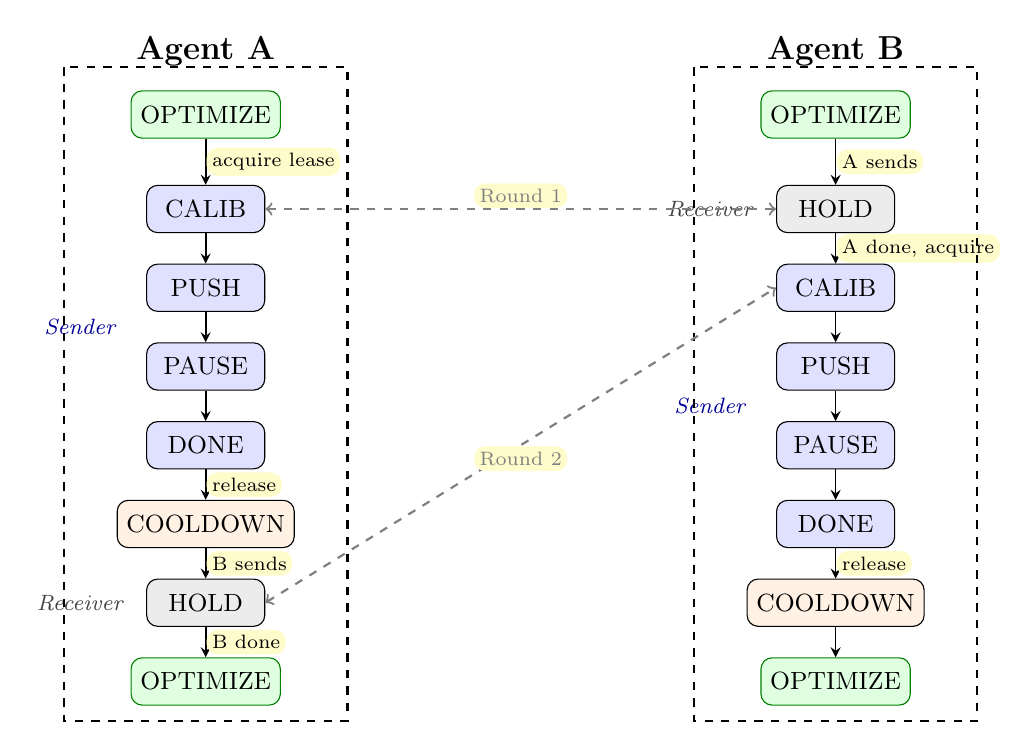
\begin{tikzpicture}[
  node distance=1.0cm,
  st/.style={rectangle, draw, rounded corners, minimum width=1.5cm, minimum height=0.6cm, font=\small},
  send/.style={st, fill=blue!12},
  recv/.style={st, fill=gray!15},
  shared/.style={st, fill=green!12, draw=green!50!black},
  cooldown/.style={st, fill=orange!10},
  arrow/.style={->, >=stealth, semithick},
  tlabel/.style={font=\scriptsize, fill=yellow!20, rounded corners, inner sep=2pt},
]

% ══ Column positions ══
\def\xa{0}
\def\xb{8}

% ══ Agent A (left) ══
\node[font=\large\bfseries] at (\xa, 1.0) {Agent A};

\node[shared] (aopt0) at (\xa, 0.2) {OPTIMIZE};
\node[send] (acalib) at (\xa, -1.0) {CALIB};
\node[send] (apush) at (\xa, -2.0) {PUSH};
\node[send] (apause) at (\xa, -3.0) {PAUSE};
\node[send] (adone) at (\xa, -4.0) {DONE};
\node[cooldown] (acool) at (\xa, -5.0) {COOLDOWN};
\node[recv] (ahold) at (\xa, -6.0) {HOLD};
\node[shared] (aopt1) at (\xa, -7.0) {OPTIMIZE};

\draw[arrow] (aopt0) -- node[tlabel, right] {acquire lease} (acalib);
\draw[arrow] (acalib) -- (apush);
\draw[arrow] (apush) -- (apause);
\draw[arrow] (apause) -- (adone);
\draw[arrow] (adone) -- node[tlabel, right] {release} (acool);
\draw[arrow] (acool) -- node[tlabel, right] {B sends} (ahold);
\draw[arrow] (ahold) -- node[tlabel, right] {B done} (aopt1);

% Sender/Receiver labels
\node[font=\footnotesize\itshape, blue!60!black] at (\xa-1.6, -2.5) {Sender};
\node[font=\footnotesize\itshape, gray!50!black] at (\xa-1.6, -6.0) {Receiver};

% Agent A box
\draw[dashed, thick] (\xa-1.8, 0.8) rectangle (\xa+1.8, -7.5);

% ══ Agent B (right) ══
\node[font=\large\bfseries] at (\xb, 1.0) {Agent B};

\node[shared] (bopt0) at (\xb, 0.2) {OPTIMIZE};
\node[recv] (bhold) at (\xb, -1.0) {HOLD};
\node[send] (bcalib) at (\xb, -2.0) {CALIB};
\node[send] (bpush) at (\xb, -3.0) {PUSH};
\node[send] (bpause) at (\xb, -4.0) {PAUSE};
\node[send] (bdone) at (\xb, -5.0) {DONE};
\node[cooldown] (bcool) at (\xb, -6.0) {COOLDOWN};
\node[shared] (bopt1) at (\xb, -7.0) {OPTIMIZE};

\draw[arrow] (bopt0) -- node[tlabel, right] {A sends} (bhold);
\draw[arrow] (bhold) -- node[tlabel, right] {A done, acquire} (bcalib);
\draw[arrow] (bcalib) -- (bpush);
\draw[arrow] (bpush) -- (bpause);
\draw[arrow] (bpause) -- (bdone);
\draw[arrow] (bdone) -- node[tlabel, right] {release} (bcool);
\draw[arrow] (bcool) -- (bopt1);

% Sender/Receiver labels
\node[font=\footnotesize\itshape, gray!50!black] at (\xb-1.6, -1.0) {Receiver};
\node[font=\footnotesize\itshape, blue!60!black] at (\xb-1.6, -3.5) {Sender};

% Agent B box (same size as A)
\draw[dashed, thick] (\xb-1.8, 0.8) rectangle (\xb+1.8, -7.5);

% ══ Lease coordination ══
% Round 1: A enters CALIB (holds lease), B observes and enters HOLD
\draw[dashed, gray, thick, <->] (acalib.east) -- node[tlabel, above] {Round 1} (bhold.west);

% Round 2: B enters CALIB (holds lease), A observes and enters HOLD
\draw[dashed, gray, thick, <->] (ahold.east) -- node[tlabel, below] {Round 2} (bcalib.west);

\end{tikzpicture}
\caption{Two-agent turn-taking in the impulse protocol. Both agents
start in OPTIMIZE. In Round 1, Agent A acquires the sender lease and
enters the detection cycle: CALIB (hold neutral, find safe perturbation
amplitude), PUSH (drive parameters to extremes), PAUSE (return to
neutral), DONE (release lease). Agent B observes the active lease
and enters HOLD as passive receiver throughout A's detection cycle.
After cooldown, the roles reverse for Round 2. CALIB encompasses
HOLD-CALIB (parameter flatness search) and IMPULSE-CALIB (adaptive
perturbation with guardrail backoff). Dashed arrows show lease
pairing: while one agent holds the sender lease, the partner is in
HOLD.}
\label{fig:state-machine}
\end{figure*}
